% ===== Appendix =====

\section{Repair Cost Distribution}\label{app:cost-dist}

\begin{figure}[h]
\centering
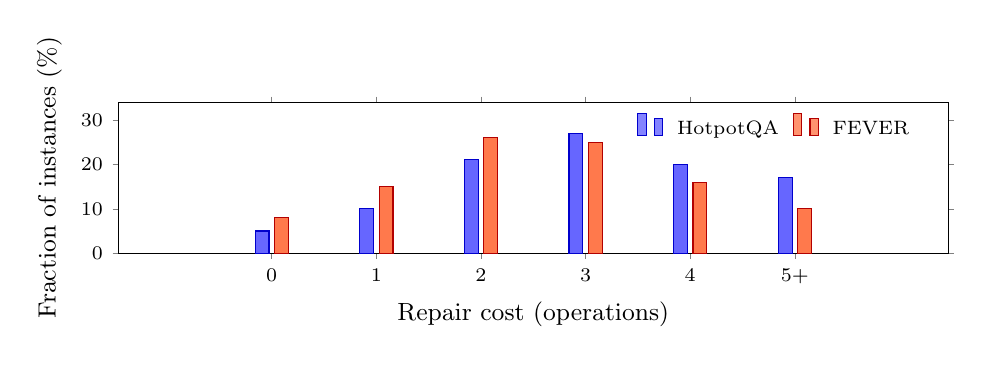
\begin{tikzpicture}
\begin{axis}[
  width=\columnwidth,
  height=3.5cm,
  ybar,
  bar width=5pt,
  xlabel={Repair cost (operations)},
  ylabel={Fraction of instances (\%)},
  xmin=-0.7, xmax=5.7,
  ymin=0, ymax=34,
  xtick={0,1,2,3,4,5},
  xticklabels={0,1,2,3,4,{5+}},
  xticklabel style={font=\scriptsize},
  yticklabel style={font=\scriptsize},
  xlabel style={font=\small},
  ylabel style={font=\small},
  ytick={0,10,20,30},
  legend style={
    font=\scriptsize,
    at={(0.97,0.97)},
    anchor=north east,
    draw=none,
    fill=white,
    fill opacity=0.8,
    text opacity=1,
    column sep=3pt,
  },
  legend columns=2,
  tick align=outside,
  major tick length=2pt,
  enlarge x limits=0.12,
]
\addplot[fill=blue!60, draw=blue!80!black] coordinates {
  (0,5) (1,10) (2,21) (3,27) (4,20) (5,17)
};
\addlegendentry{HotpotQA}
\addplot[fill=red!50!orange!70, draw=red!70!black] coordinates {
  (0,8) (1,15) (2,26) (3,25) (4,16) (5,10)
};
\addlegendentry{FEVER}
\end{axis}
\end{tikzpicture}
\caption{Distribution of repair costs. 83\% of HotpotQA and 90\% of FEVER repairs require at most 4~operations, confirming that \textsc{Argus} achieves targeted, minimal-change edits.}
\label{fig:cost-dist}
\end{figure}

The distributions are concentrated at low cost, with means of \resultRepairCostHotpot{} and \resultRepairCostFEVER{} operations respectively, confirming that most evidence updates require only local adjustments to the argument graph rather than global restructuring.

\section{Qualitative Repair Example}\label{app:repair-example}

\begin{figure}[h]
\centering
\begin{tikzpicture}[node distance=0.8cm and 0.8cm,
  lbl/.style={font=\small\bfseries, anchor=south}]
  % --- Before ---
  \node[lbl] at (0, 1.7) {Before};
  \node[acc node] (b1) at (-0.55, 0.85) {$b_1$};
  \node[acc node] (b2) at (0.55, 0.85) {$b_2$};
  \node[rej node] (b3) at (-0.55, 0) {$b_3$};
  \node[rej node, tgt node] (bt) at (0.55, 0) {$b_t$};
  \node[new node] (b5) at (0, -1.15) {$b_5$};
  \draw[att edge] (b5) -- (b3);
  \draw[att edge] (b5) -- (bt);
  % --- Arrow ---
  \draw[-{Stealth[length=2.5mm]}, very thick, gray!60] (1.4, 0.4) -- (1.95, 0.4);
  % --- After Argus ---
  \node[lbl] at (3.2, 1.7) {\textsc{Argus}};
  \node[acc node] (a1) at (2.65, 0.85) {$b_1$};
  \node[acc node] (a2) at (3.75, 0.85) {$b_2$};
  \node[acc node] (a3) at (2.65, 0) {$b_3$};
  \node[acc node, tgt node] (at) at (3.75, 0) {$b_t$};
  \node[rej node] (a5) at (3.2, -1.15) {$b_5$};
  \node[new node] (a6) at (4.3, -1.15) {$b_6$};
  \draw[att edge] (a5) -- (a3);
  \draw[att edge] (a5) -- (at);
  \draw[att edge, NewBlue!80!black, line width=1.1pt] (a6) -- (a5);
  \node[font=\scriptsize, text=AccGreen!70!black] at (3.2, -1.75) {cost = 2};
\end{tikzpicture}
\caption{A HotpotQA repair example. \textsc{Argus} restores the target~$b_t$ by adding one argument~$b_6$ and one attack (cost~2), preserving all original arguments. Self-Refine regenerates 5 of 6 units.}
\label{fig:repair-example}
\end{figure}

Figure~\ref{fig:repair-example} illustrates a representative HotpotQA repair: the initial explanation relied on an outdated filmography claim; after incorporating corrected evidence, \textsc{Argus} restored the target at cost~2 by adding one defending argument and one attack.
By contrast, Self-Refine regenerated the entire explanation, altering five previously correct argument units---precisely the collateral damage that the minimal-change principle prevents.

\section{Sensitivity Analysis}\label{app:sensitivity}

Pilot studies on 100 HotpotQA instances explore three design choices.
Confidence-weighted and structure-preserving ($w{=}2$) cost models shift repairs toward augmentation (34--51\% fewer deletions) while maintaining faithfulness and repair accuracy within 1 percentage point of uniform cost, confirming that the cost model affects repair \emph{style} rather than \emph{quality}.
Varying the NLI threshold from 0.5 to 0.9 shows faithfulness is stable (0.839--0.851) while repair cost rises from 2.4 to 4.1; 0.7 balances these factors.
Repair optimality rises from 87.2\% ($k{=}1$) to 99.7\% ($k{=}3$) and plateaus, confirming $k{=}3$ as the operating point.
Using Llama-3-70B-Instruct as the extraction backbone yields faithfulness 0.813 and contestability 0.762 (vs.\ \resultFaithHotpot{}/\resultContestHotpot{} for GPT-4o), with comparable repair accuracy (0.867) and cost (3.4); the gap is attributable to noisier extraction rather than the repair mechanism.

\section{Error Analysis}\label{app:error-analysis}

Among the 0.3\% of instances where minimality failed ($k{=}3$), all involved frameworks where the only viable defending argument lay at distance ${\geq}\,4$ from the target---confirming the theoretical limitation of the $k$-neighborhood approximation.
Repair accuracy below 1.0 arises when the LLM-generated explanation has structural errors that propagate through extraction: even after restoring the target argument's acceptability, the underlying answer may remain incorrect if the original decomposition was flawed.
